\subsection{Kammerha}
Under J60 gav \alkymia \TKET et kalaha spil som gave, så man kunne spille deres dødskalaha, som \alkymia havde navngivet ``kammerha'', da de forbandt det med \TKET. Formålet med spillet er at skyde en kalaha kugle i bordet og prøve at ramme et af modstanderens kar på den modsatte side af kalaha-pladen.

Målet er at få fordelt 14 kugler i modstanderens 6 kar, hvor kuglerne som følgende fordelingen $(1, 2, 4, 4, 2, 1)$. Til spillet skal man bruge: 1 styks kalaha spil og 34 kalaha kugler (14 kugler + 3 ekstra til hvert hold). Man kan spille 1v1 eller 2v2\footnote{Eller enhver kombination af de to.}. 

{\par \centering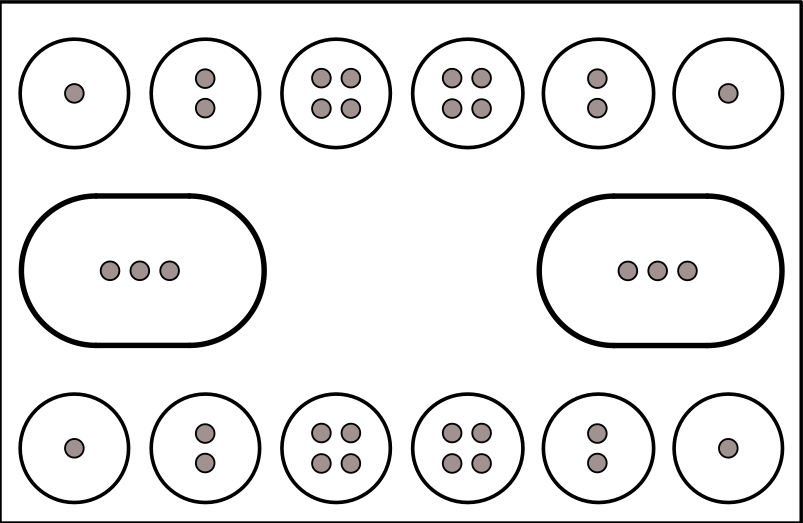
\includegraphics[height=4cm]{../img/kammerha.png} \par}

Oftest starter man med at lægge alle kugler ud i de korrekte kar, som vist billedet: (1, 2, 4, ,4 , 2, 1) og 3 ekstra kugler i hvert Ta'-kar. Ens eget Ta'-kar er det til højre for en selv.
For at finde ud af hvilket holder der skal starte, tager én spiller fra hvert hold en kugle og kigger modspilleren dirgonalt overfor dybt i øjene, tæller ned fra 3 og skyder. Det hold der har ramt det bedste skud starter. Hvis begge spillere misser eller begge rammer det samme kar gentages processen med spillerne der sidder på den anden dirgonal.

Når startholdet er funder, skiftes man da til at skyde en kugle i bordet og prøve at ramme modstandernes kar. Hvis man rammer i et af modstanderens kar, må man skyde igen indtil man ikke rammer et kar. Spillet afsluttes ved at der minimum er (1, 2, 4, 4, 2, 1) kugler fordelt på modstanderens kar, som på billedet, og holdet der har opnået sluttilstanden, erklæres vindere. Hvis begge sider løber tør for kugler erklæres spillet for uafgjort.

Der er nogle specielle regler: 
\begin{itemize}
    \item Hvis man rammer i modstanderens Ta'-kar, må de beholde kuglen og det bliver deres tur. 
    \item Hvis man rammer i ens eget Ta'-kar beholder man selv kuglen men ens tur er slut. 
    \item Hvis du skyder bolden i bordet og den ikke rammer pladen overhovedet\footnote{Hvis kuglen rammer siderne af pladen, så tæller skuddet stadig.} så tæller skuddet ikke og du må skyde igen. 
\end{itemize}

Ydermere er der nogle specielle regler omkring drikkevare:
\begin{itemize}
    \item Man drikker hver gang en modstander rammer i ens kar, med følgende mængder alt efter hvilket kar de rammer:
    \begin{itemize}
        \item De to yderste kar $\rightarrow$ 4 tåre pr. kugle.
        \item De to næstyderset kar $\rightarrow$ 2 tåre pr. kugle.
        \item De to inderste kar $\rightarrow$ 1 tår pr. kugle.
    \end{itemize}
    \item Antallet af tårer summeres, så hvis der bliver skudt én kugle i det yderste kar og to kugler i en af de inderste kar, så skal man drikke $4 + 1 = 5$ tåre\footnote{Dette antal tåre deles ligeligt mellem spillere på holdet der drikker. Dog rundes der op, for eksempelt vil 5 tåre fordelt på 2 spillere betyder at hver drikker 3 tåre.}.
\end{itemize}